% (c) 2017 Leonardo Aldegheri
% (c) 2017 Carlotta Gualtieri

\chapter{Topologia della retta}

\section{La topologia della retta}
%label{}
Già dall'etimologia del termine, dal greco ``\emph{topos}'' che significa 
``luogo'', apprendiamo che il termine topologia indica lo studio ragionato 
dei luoghi. Nell'ambito dei nostri studi la topologia, o scienza dei luoghi, 
è quella branca della matematica che studia le proprietà geometriche delle 
figure piane e spaziali che restano inalterate eseguendo trasformazioni 
biunivoche. In particolare, con l'espressione topologia della retta si indica 
lo studio della retta come insieme di punti, approfondendo i concetti di 
vicinanza, lontananza e distanza tra di essi.\\

Il primo passo che facciamo è quello di identificare i numeri reali con i 
punti della retta: ad ognuno degli infiniti punti della retta facciamo 
corrispondere uno degli infiniti numeri dell'insieme $\mathbb{R}$. Ricordiamo 
infatti che entrambi sono insiemi ordinati e completi e possiamo costruire 
una corrispondenza biunivoca tra i loro elementi, fissando sulla retta 
un'origine e un verso di percorrenza, come ci consente di fare il postulato 
di ordinamento sulla retta.\\

Identificando i numeri reali con i punti della retta, possiamo definire la 
distanza tra due numeri $x$ e $y$ reali come la distanza $d(x, y)$ tra i 
punti che li rappresentano. Con $x$, $y\in\mathbb{R}$ la distanza è data da:
\begin{equation}
%\label{eq:}
  d(x,y)=\sqrt{(x-y)^2}=\vert x-y\vert
\end{equation}
ed ha le seguenti proprietà:
\begin{enumerate}
  \item $\forall x,\,y \in A,\,d(x,y)=d(y,x)$ cioè la distanza è 
simmetrica,
  \item $\forall x,\,y \in A,\,d(x,y)\geq0$,
  \item $d(x,y)=0\Leftrightarrow x=y$,
  \item $\forall x,\,y,\,z \in A,\,d(x,y)\leq d(x,z)+d(z,y)$ detta 
disuguaglianza triangolare.
\end{enumerate}

\section{Gli intervalli}
%label{}
  \begin{definizione}
Un \textsc{intervallo} è un sottoinsieme di $\mathbb{R}$, formato da tutti i 
reali compresi tra due estremi, finiti o infiniti.\\
\end{definizione}

Gli intervalli possono essere chiusi o aperti a seconda che gli estremi 
appartengano o meno all'intervallo.\\
Gli intervalli possono essere limitati se entrambi i loro estremi sono 
finiti: segmenti o illimitati se un estremo non è finito: semirette.

\textcolor{red}{TABELLA INTERVALLI da rifare o vedi quella a vol.2 pag.\dots}
\begin{figure}[htpb!]
  \centering
  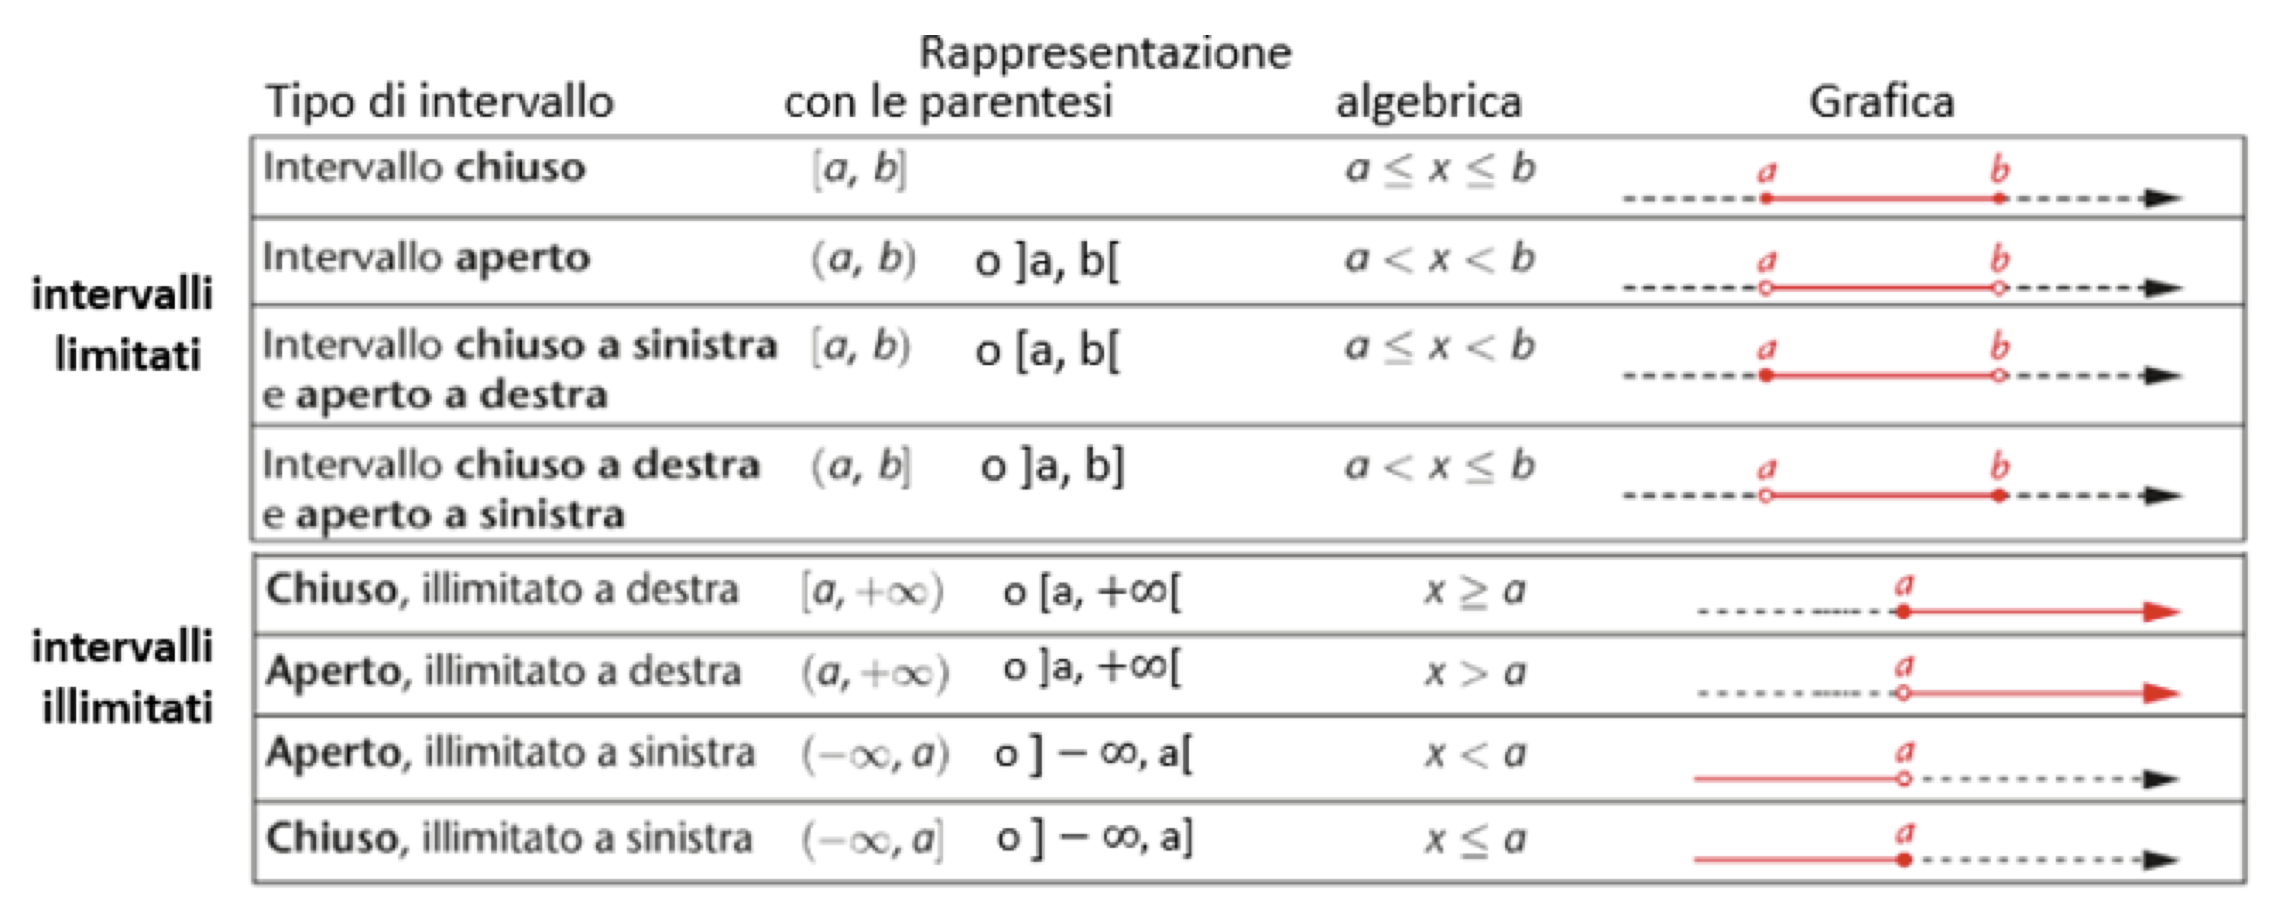
\includegraphics[width=1\textwidth]{img/top_tab.png}%\caption{}
  %\label{fig:funz_14abc}
\end{figure}




\begin{esempio} Intervalli finiti e infiniti: metodi di scrittura.
  \begin{itemize}
  \item[a)] L'insieme $\mathbb{R}$ si può scrivere come 
l'intervallo $]-\infty, +\infty[$\\
  \item[b)] L'insieme $\mathbb{R}-\{3\}$ si può indicare con 
l'intervallo $]-\infty, 3[\,\cup\,]3,+\infty[$\\
  \item[c)] L'insieme $\mathbb{R}-\{-2,3\}$ si può indicare con 
$]-\infty, -2[\,\cup\,]-2,3[\,\cup\,]3,+\infty[$\\
  \item[d)] L'insieme delle soluzioni della disequazione 
$x^2+3x>0$ si può scrivere come $]-\infty,-3[\,\cup\,]0,+\infty[$.\\
  \end{itemize}
\end{esempio}
  
Per quanto riguarda le operazioni tra intervalli evidenziamo che l'unione di 
intervalli aperti è un insieme aperto; l'intersezione di due intervalli 
aperti è un aperto. L'intersezione di intervalli chiusi è un intervallo 
chiuso; l'unione di un numero finito di intervalli chiusi è chiuso. Un 
intervallo $B$ è chiuso se il suo complementare è aperto.\\

Grazie alla corrispondenza tra numeri reali e punti di una retta, per 
indicare un elemento di un intervallo possiamo riferirci indifferentemente a 
un numero o un punto.

%
%
\section{Gli intorni}
%label{}
  \begin{definizione}
Si definisce intorno o intorno completo di un numero reale $x_0$, o punto 
$x_0$, un qualsiasi intervallo aperto contenente $x_0$.\\
  \end{definizione}

Rappresentiamo in simboli e graficamente un intorno
\begin{equation}
%\label{eq:}
I(x_0)=]x_0-\delta_1,x_0+\delta_2[
\end{equation}
con $\delta_1$ e $\delta_2$ reali positivi, cioè $\delta_1,\,\delta_2 \in 
\mathbb{R^+}$, o equivalentemente
\begin{equation}
%\label{eq:}
I(x_0)=\{x\in \mathbb{R}\,\vert\,x_0-\delta_1<x<x_0+\delta_2\}
\end{equation}
  \begin{figure}[htpb!]
  \centering
  
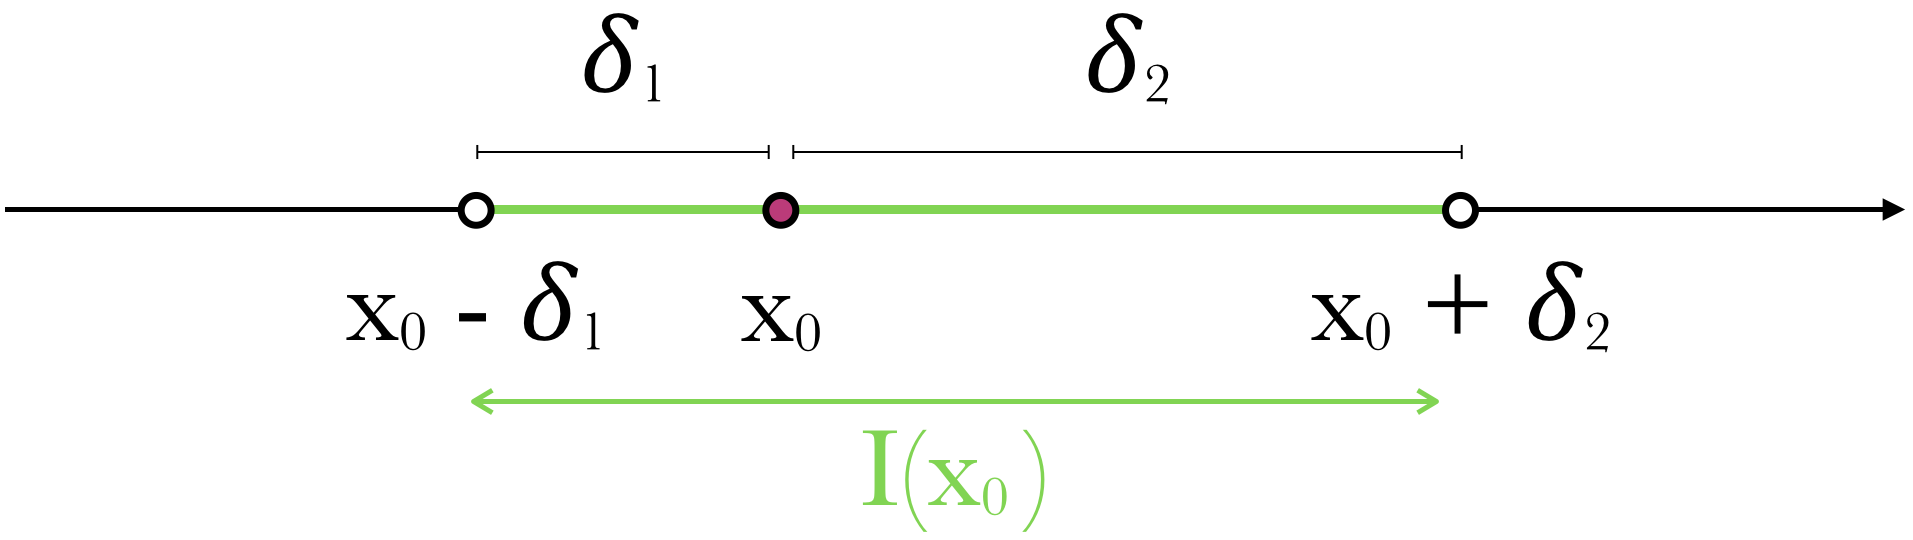
\includegraphics[width=0.5\textwidth]{img/top_1.png}%\caption{}
  %\label{fig:funz_14abc}
  \end{figure}
  
Da quanto visto risulta chiaro che per ogni numero reale, esistono infiniti 
intorni.\\
Per quanto riguarda le operazioni associabili agli intorni è da sottolineare 
che l'intersezione e l'unione di due o più intorni di $x_0$ sono ancora 
intorni di $x_0$.\\

\begin{figure}[htpb!]
\centering
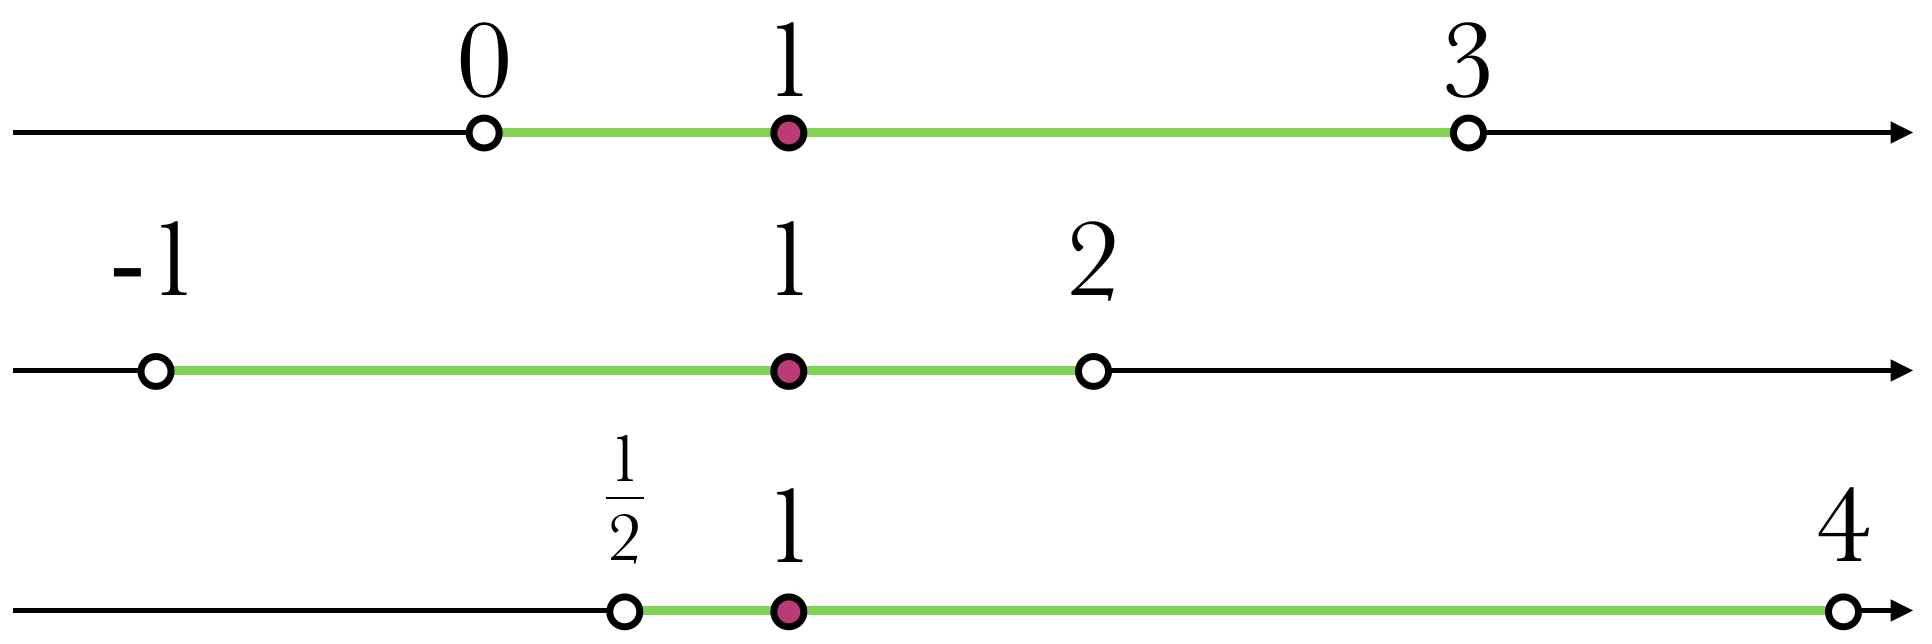
\includegraphics[width=0.5\textwidth]{img/top_7.png}%\caption{}
%\label{fig:funz_14abc}
  \end{figure}
  
Chiarito il concetto di intorno, introduciamo alcune particolari tipologie di 
intorno che renderanno più funzionale l'uso di questo concetto. Vedremo 
l'intorno circolare, l'intorno destro e l'intorno sinistro.\\

\begin{definizione}
  Dato un numero reale $x_0$ e un numero reale positivo $\delta$, si 
definisce \textsc{intorno circolare} di $x_0$, di raggio $\delta$, 
l'intervallo aperto $I_C(x_0)$ di centro $x_0$ e raggio $\delta$.\\
\end{definizione}

\begin{equation}
  I_C(x_0)=]x_0-\delta,\,x_0+\delta[
\end{equation}
o equivalentemente
 \begin{equation}
  I_C(x_0)=\{x\in \mathbb{R}\,\vert\,\vert x-x_0\vert<\delta\}
\end{equation}

\begin{figure}[htpb!]
  \centering
  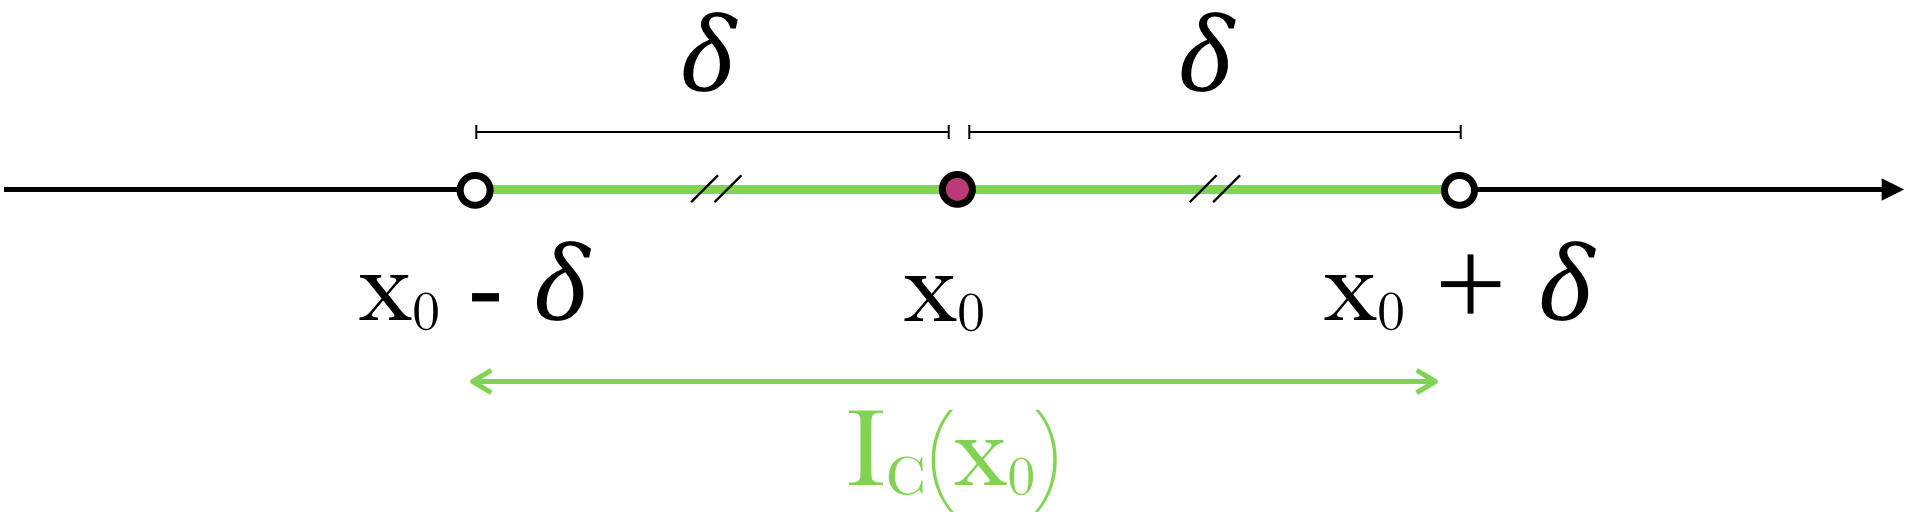
\includegraphics[width=0.5\textwidth]{img/top_2.png}%\caption{}
  %\label{fig:funz_14abc}
\end{figure}


\begin{definizione}
  Si dice intorno sinistro del numero reale $x_0$, $I_s(x_0)$ o 
$I^-(x_0)$, un qualsiasi intervallo aperto avente $x_0$ come estremo destro. 
$\delta\in\mathbb{R}$ è detta ampiezza.\\
\begin{equation}
  I_s(x_0)=]x_0-\delta,\,x_0[
\end{equation}
o equivalentemente
\begin{equation}
  I_s(x_0)=\{x\in \mathbb{R}\,\vert\, x_0-\delta < x<x_0\}
\end{equation}
\end{definizione}

\begin{figure}[htpb!]
  \centering
  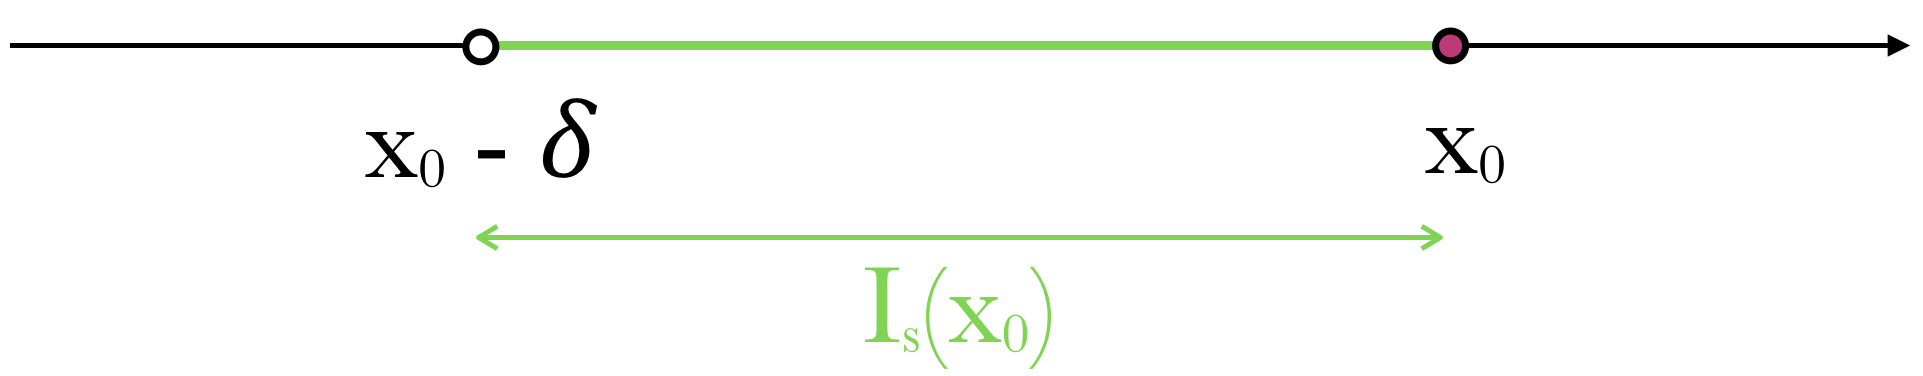
\includegraphics[width=0.5\textwidth]{img/top_3.png}%\caption{}
  %\label{fig:funz_14abc}
\end{figure}

\begin{definizione}
  Si dice intorno destro del numero reale $x_0$, $I_d(x_0)$ o 
$I^+(x_0)$, un qualsiasi intervallo aperto avente $x_0$ come estremo 
sinistro. $\delta\in\mathbb{R}$ è detta ampiezza.\\
\begin{equation}
  I_d(x_0)=]x_0,\,x_0+\delta[
\end{equation}
o equivalentemente
\begin{equation}
  I_d(x_0)=\{x\in \mathbb{R}\,\vert\, x_0 < x<x_0+\delta\}
\end{equation}
\end{definizione}

\begin{figure}[htpb!]
  \centering
  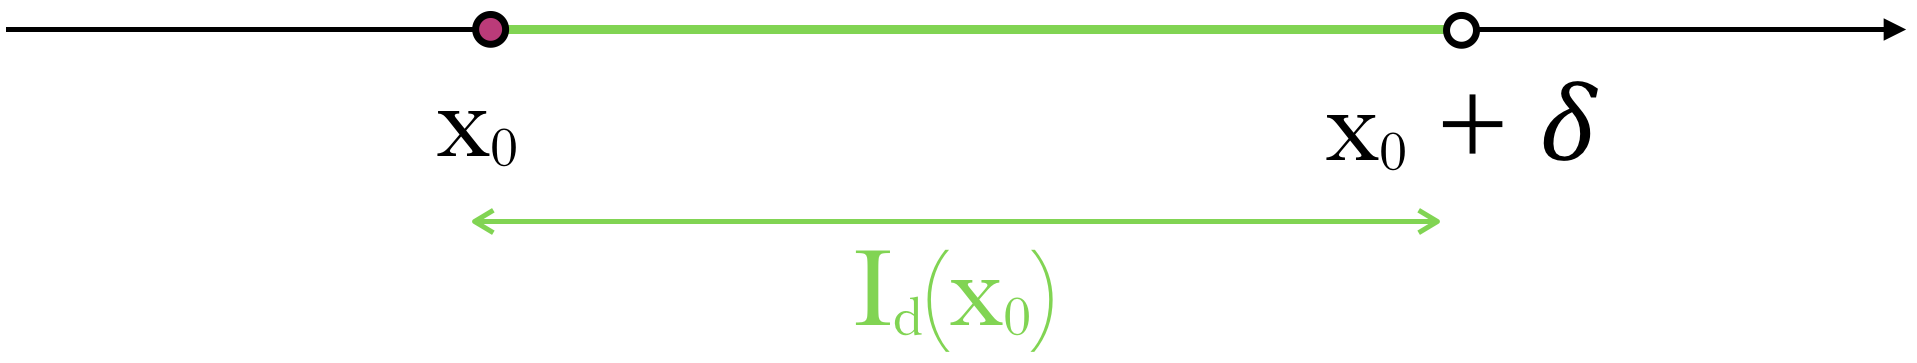
\includegraphics[width=0.5\textwidth]{img/top_4a.png}%\caption{}
  %\label{fig:funz_14abc}
\end{figure}

\begin{esempio} Intorni e intervalli.
\begin{itemize}
  \item[a)] L'intervallo $]-2, 9[$ è un intorno di $x_0=4$; rispetto a 
$x_0=4$ non sono intorni né $]5, 9[$ né $[3, 5]$.\\
  \item[b)] L'intervallo $]0, 6[$ è un intervallo circolare di $x_0=3$ 
di raggio $\delta=3$.\\
  \item[c)] L'intervallo $]\frac{4}{5},1[$ è un intorno sinistro di $1$ 
di ampiezza $\frac{1}{5}$. \\
\end{itemize}
\end{esempio}

\section{Insiemi limitati e illimitati}
%label{}
Consideriamo un insieme non vuoto $A\subset \mathbb{R}$. L'insieme A si dice 
superiormente limitato se esiste un numero $\alpha \in \mathbb{R}$ maggiore o 
uguale a tutti gli elementi di $A$, cioè $x\leq\alpha$ , $\forall x\in A$. 
Tale numero prende il nome di maggiorante, un insieme superiormente limitato 
ammette infiniti maggioranti. Se un insieme $A$ non è superiormente limitato 
si dice superiormente illimitato.\\
In simboli:\\

$A$ è \textsc{superiormente limitato} se 
\begin{equation}
  \exists \alpha\in\mathbb{R}\, \vert\, \forall x \in A,\,\alpha\geq x
\end{equation}
\\

$A$ è \textsc{superiormente illimitato} se 
\begin{equation}
  \forall M\in\mathbb{R},\, \exists x \in A\, \vert\,x> M
\end{equation}

Specularmente l'insieme $A$ si dice inferiormente limitato se esiste un 
numero $\beta\in \mathbb{R}$ minore o uguale a tutti gli elementi di $A$, 
cioè $x\geq\beta$ , $\forall x\in A$. Tale numero prende il nome di 
minorante, un insieme inferiormente limitato ammette infiniti minoranti. Se 
un insieme $A$ non è inferiormente limitato si dice inferiormente illimitato.
In simboli:\\

$A$ è \textsc{inferiormente limitato} se 
\begin{equation}
  \exists \beta\in\mathbb{R}\, \vert\, \forall x \in A,\,\beta\leq x
\end{equation}
\\

$A$ è \textsc{inferiormente illimitato} se 
\begin{equation}
  \forall m\in\mathbb{R},\, \exists x \in A\, \vert\,x< m
\end{equation}
Infine, completiamo la trattazione appena fatta notando che l'insieme $A$ si 
dice limitato se è sia inferiormente limitato che superiormente limitato, 
esiste cioè un intervallo limitato che lo contiene. Un insieme illimitato 
superiormente e inferiormente si dice illimitato.\\

\begin{esempio} Limitatezza/illimitatezza di insiemi, maggioranti e minoranti.
\begin{itemize}
  \item[a)] L'insieme $A=]-\infty,4[ \cup [8,15]$ è superiormente 
limitato, perché tutti i suoi elementi sono minori o uguali a 15. 15 è un 
maggiorante, ma anche 16, 20 e 204 lo sono. $A$ è, poi, inferiormente 
illimitato.\\
  \item[b)] L'insieme $B=\{5\}\cup]9,+\infty[$ è inferiormente limitato 
e tutti i numeri minori o uguali a 5 sono minoranti; l'insieme è 
superiormente illimitato.\\

  \item[c)] L'insieme $C=\{x\in\mathbb{R}\vert 
x=\frac{1}{n},\,n\in\mathbb{N}-\{0\}\}=\{1,\frac{1}{2},\frac{1}{3}
,\dots\}$ è limitato, ha 1 come maggiorante e 0 come minorante. Altri 
minoranti ad esempio sono $-3$, $-5$ ecc, altri maggioranti 5, 8 ecc.\\

  \item[d)] L'insieme $D=]3,5]\cup[7,9[$ ammette 2 come minorante e 10 
come maggiorante, quindi è sia inferiormente che superiormente limitato: $D$ 
è limitato.\\

  \item[e)] L'insieme $\mathbb{Q}$ non ammette né minoranti né 
maggioranti, quindi non è non è limitato né inferiormente né superiormente.\\
\end{itemize}
\end{esempio}

Avendo introdotto gli insiemi illimitati possiamo ora parlare degli intorni 
di infinito. Anche se $+\infty$ e $-\infty$ non sono numeri reali è utile 
introdurne gli intorni.\\

\begin{definizione}
  Dati $a,\,b\in\mathbb{R}$ con $a<b$, definiamo \textsc{intorno di 
meno infinito} un qualsiasi intervallo illimitato a sinistra e aperto a destra
\begin{equation}
  I(-\infty)=]-\infty,a[=\{x\in\mathbb{R}\vert x<a\}
\end{equation}
\end{definizione}

\begin{figure}[htpb!]
  \centering
  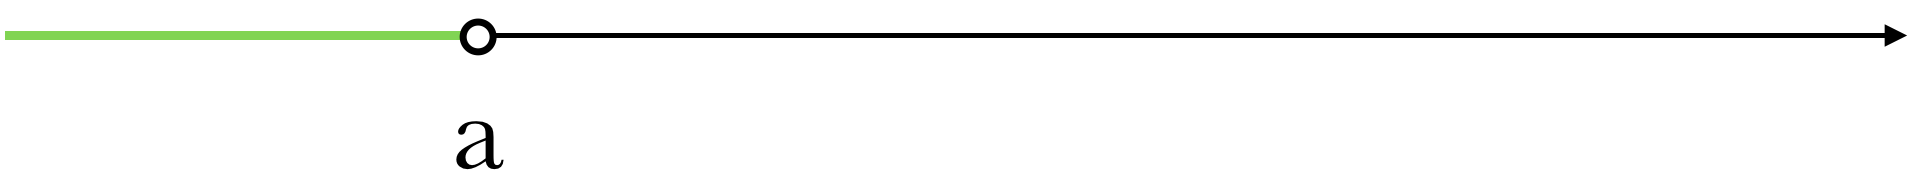
\includegraphics[width=0.5\textwidth]{img/top_4.png}%\caption{}
  %\label{fig:funz_14abc}
\end{figure}


\begin{definizione}
  Dati $a,\,b\in\mathbb{R}$ con $a<b$, definiamo \textsc{intorno di più 
infinito} un qualsiasi intervallo illimitato a destra e aperto a sinistra
\begin{equation}
  I(+\infty)=]b,+\infty[=\{x\in\mathbb{R}\vert x>b\}
\end{equation}
\end{definizione}

\begin{figure}[htpb!]
  \centering
  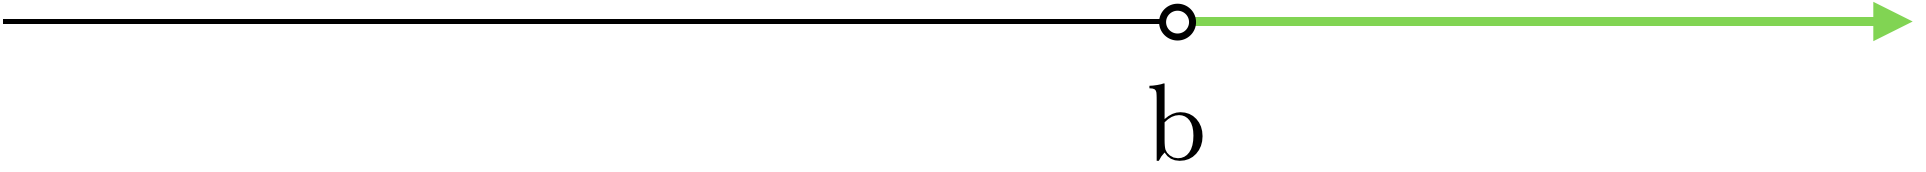
\includegraphics[width=0.5\textwidth]{img/top_5.png}%\caption{}
  %\label{fig:funz_14abc}
\end{figure}

\begin{definizione}
  Dati $a,\,b\in\mathbb{R}$ con $a<b$, definiamo \textsc{intorno di 
infinito} l'unione tra un intorno di $-\infty$  e un intorno di $+\infty$ 
\begin{equation}
  I(\infty)=I(-\infty)\cup I(+\infty)=\{x\in\mathbb{R}\vert x<a \lor 
x>b\}
\end{equation}
e \textsc{l'intorno circolare di infinito}, dove $c\in\mathbb{R}^+$ come
\begin{equation}
  I_c(\infty)=]-\infty,-c[\cup]c,+\infty[
\end{equation}
\end{definizione}

\begin{figure}[htpb!]
  \centering
  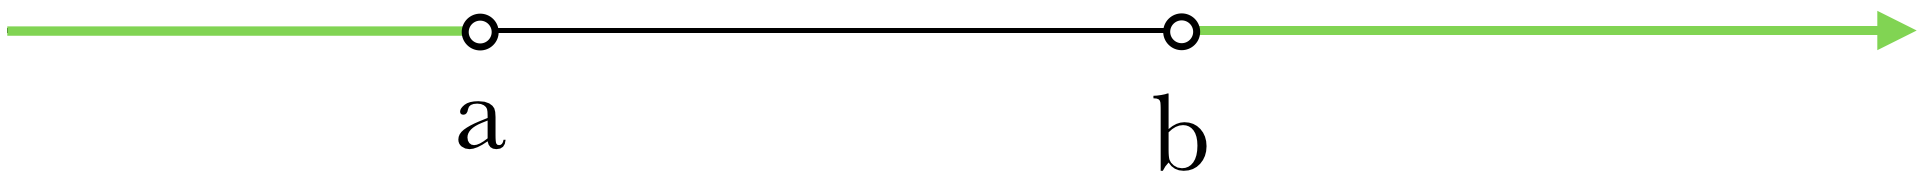
\includegraphics[width=0.5\textwidth]{img/top_6.png}%\caption{}
  %\label{fig:funz_14abc}
\end{figure}


\begin{esempio} Scrivere gli intervalli risultato di una disequazione come 
intorni di infiniti.
\begin{itemize}
  \item[a)] Le soluzioni della disequazione $x+4>0$ formano un intorno 
di $+\infty$.  Soluzioni: $x>-4$, $I(+\infty)=]-4, +\infty[$.\\
  \item[b)] Le soluzioni della disequazione $x^2+5x+6>0$ formano un 
intorno di infinito. Soluzioni: $-3<x\lor x>-2$, $I(\infty)=]-\infty, -3[ 
\cup]-2, +\infty[$.\\
  \item[c)] Consideriamo la disequazione $\vert x\vert>3$, le soluzioni 
forniscono un esempio di intorno circolare di $\infty$ che è 
$I_c(\infty)=]-\infty,-3[\cup]3,+\infty[$.
\end{itemize} 
\end{esempio}

\section{Massimi, minimi ed estremi}
%label{}
Ragioniamo ora su quanto appena visto, nel precedente paragrafo. Se un 
insieme $A$ è superiormente limitato ha infiniti maggioranti; si può allora 
individuare un insieme di maggioranti, tra i quali non è identificabile un 
maggiorante più grande di tutti, mentre possiamo pensare a un maggiorante più 
piccolo di tutti.\\

Questo maggiorante viene chiamato estremo superiore di $A$, se tale punto è 
anche compreso in $A$ prende il nome di massimo. Chiaramente potremmo fare un 
discorso analogo per i minoranti, individuando il maggiore tra di essi, detto 
estremo inferiore. Se l'estremo inferiore appartiene all'insieme che si sta 
studiando, prende il nome di minimo. Entriamo nel merito delle definizioni.\\

\begin{definizione}
  Un numero reale $M$ si dice massimo di $A$, $\max{A}$, se appartiene 
ad $A$ ed è un maggiorante di $A$.\\
\end{definizione}

\begin{definizione}
  Un numero reale $m$ si dice minimo di $A$, $\min{A}$, se appartiene 
ad $A$ ed è un minorante di A.\\
\end{definizione}

\begin{definizione}
  Si definisce $S$ estremo superiore di $A$, $\sup{A}$, se esiste, il 
minimo dell'insieme dei maggioranti.\\
\end{definizione}

\begin{definizione}
  Si definisce $s$ estremo inferiore di $A$, $\inf{A}$, se esiste, il 
massimo dell'insieme dei minoranti.\\
\end{definizione}

\begin{esempio}Studiamo i massimi e i minimi dei seguenti intervalli.\\
Consideriamo l'intervallo chiuso $[0,2]$, esso presenta un minimo in 0 e un 
massimo in 2, se prendiamo invece l'intervallo aperto $]0,2[$ esso non avrà 
né massimo né minimo, perché né 0 né 1 appartengono all'insieme. Risulta 
chiaro quindi che nell'intervallo aperto solo a destra $[0,2[$ sarà presente 
un minimo, cioè 0, ma non un massimo.\\
\end{esempio}

\begin{esempio}Studiamo gli estremi superiore ed inferiore dei seguenti 
intervalli.\\
Consideriamo l'intervallo $A=]1, 5]$, aperto a sinistra e chiuso a destra. 
L'intervallo ha un estremo inferiore in 1, infatti questo valore è il massimo 
dei minoranti, 1 però non è minimo in quanto non compreso in $A$. Lo stesso 
intervallo ha estremo superiore in 5, che, essendo compreso, è anche massimo. 
Notiamo che l'insieme dei maggioranti di $A$ è infatti l'insieme 
$\{x\in\mathbb{R}\vert x\geq5\}$, l'insieme dei minoranti è 
$\{x\in\mathbb{R}\vert x\leq1\}$.\\
Consideriamo ora l'intervallo $B=\{x\in\mathbb{R}\vert x<3\}$, non essendo 
inferiormente limitato $B$ non presenta né estremo inferiore né minimo. 
L'estremo superiore di $B$ è 3, che non essendo compreso non è massimo.\\
\end{esempio}

Soffermiamoci ancora sui concetti di $\sup$, estremo superiore, e di $\inf$, 
estremo inferiore, enunciando la seguente proprietà che precisa l'esistenza e 
l'unicità di $\sup$ e $\inf$ negli insiemi limitati:\\

Sia $A\subset\mathbb{R}$, non vuoto:
\begin{itemize}
  \item se $A$ è superiormente limitato allora esiste in $\mathbb{R}$ 
l'estremo superiore di $A$ $\sup{A}$ ed è unico.
  \item se $A$ è inferiormente limitato allora esiste in $\mathbb{R}$ 
l'estremo inferiore di $A$ $\inf{A}$ ed è unico.
\end{itemize}

\section{I punti di accumulazione}
%label{}
Pensiamo ad un intervallo dato dall'insieme $A=]3, 5[$ e ad un insieme fatto 
invece di singoli punti $B=\{2,3,4,5,6\}$ e ragioniamo sul fatto che nel 
primo insieme preso un qualsiasi punto ad esempio 4, ci sarà sempre un 
intorno di 4 che contiene altri punti di $A$; anche se prendiamo in 
considerazione 3, che a dire la verità, non fa parte di A, potrei prendere un 
intorno qualsiasi di 3 e verificare che vi è almeno un punto di $A$. Questa 
riflessione non si può applicare invece all'insieme $B$, perché se prendo un 
intorno di 3, nella fattispecie un intorno circolare di raggio $\frac{1}{2}$, 
in quell'intorno non sono compresi altri punti di $B$ perché gli elementi di 
$B$ più vicini a 3 sono 2 e 4.\\

Stiamo provando ad illustrare il concetto di contiguità che gli elementi di 
un insieme mostrano, mentre gli elementi di altri insiemi non mostrano. Siamo 
pronti per la definizione di punto di accumulazione.\\

\begin{definizione}
  Dato $A$ sottoinsieme di $\mathbb{R}$, definiamo $x_0$ punto di 
accumulazione di $A$ se ogni intorno di $x_0$ contiene almeno un elemento di 
$A$ diverso da $x_0$.
\begin{itemize}
  \item[$\rhd$] Un punto di accumulazione di un insieme può appartenere 
o non appartenere all'insieme stesso.
  \item[$\rhd$]   Si può dimostrare che se $x_0$ è punto di 
accumulazione di $A$, in ogni intorno di $x_0$ devono cadere infiniti 
elementi di $A$. Consegue da questo che un insieme finito è privo di punti di 
accumulazione.
  \item[$\rhd$] L'insieme costituito dai punti di accumulazione di $A$ 
si chiama insieme derivato: $Der A$.
\end{itemize}
\end{definizione}

Come abbiamo visto nell'introduzione a questo paragrafo non tutti i punti si 
comportano come 4 per l'insieme $A$, cioè sono di accumulazione; possono 
esserci anche punti che si comportano come 3, per l'insieme $B$, cioè sono 
isolati.\\

\begin{definizione}
  Un punto $x_0$ che appartiene ad $A$ ma non è di accumulazione per $A$ 
si dice isolato. $x_0\in A$ è un punto isolato di $A$ se esiste almeno un 
intorno $I$ di $x_0$ che non contiene altri elementi di $A$ diversi da 
$x_0$.\\
\end{definizione}

Un sottoinsieme $A$ di $\mathbb{R}$ si dice \textsc{discreto} se non contiene 
nessuno dei suoi punti di accumulazione. $A$ è discreto se e solo se è 
formato da punti isolati.\\
Un insieme $B$ si dice \textsc{denso} in sé se ogni suo punto è di 
accumulazione per esso, cioè se $B\subseteq Der B$.\\

Dato $X\subset \mathbb{R}$ classifichiamo i punti di $\mathbb{R}$ 
relativamente ad $X$:
\begin{itemize}
  \item I punti interni di $X$ sono quelli che appartengono a $X$ e 
possiedono un intorno interamente contenuto in $X$.
  \item   I punti esterni ad $X$ sono quelli che non appartengono a $X$ 
e possiedono un intorno completamente disgiunto da $X$.
  \item   I punti di frontiera di $X$ hanno la proprietà che ogni loro 
intorno contiene sia punti di $X$ che punti che non appartengono a $X$.
\end{itemize}

\begin{esempio}
Relazione fra l'appartenenza di un punto all'insieme e l'essere di 
accumulazione per quell'insieme.
\begin{itemize}
  \item[a)] $x_0$ appartiene ad $A$, $x_0$ è di accumulazione per $A$\\
 $\longrightarrow$ $A=]4,8[$, $x_0=5\rightarrow x_0\in A$ ed è di 
accumulazione.
  \item[b)]  $x_0$ non appartiene ad $A$, $x_0$ è di accumulazione per 
$A$\\
 $\longrightarrow$ $A=]4,8[$, $x_0=4\rightarrow x_0\notin A$ ed è di 
accumulazione.
  \item[c)]  $x_0$ non appartiene ad $A$, $x_0$ non è di accumulazione 
per $A$\\
 $\longrightarrow$ $A=]4,8[$, $x_0=2\rightarrow x_0\notin A$ e non è di 
accumulazione.
  \item[d)] $x_0$ appartiene ad $A$, $x_0$ non è di accumulazione per 
$A$\\
  $\longrightarrow$ $A=]4,8[$, $x_0=9\rightarrow x_0\in A$ e non 
è di accumulazione.
\end{itemize}
\end{esempio}

\begin{esempio}
Studio dei punti di accumulazione.
\begin{itemize}
  \item[a)] L'insieme $A=\{ 5,6,7,8\}$ essendo finito non ha punti di 
accumulazione.
  \item[b)] Consideriamo l'insieme $C=]1,6[\,\cup\,]6,8]$
  \begin{itemize}
  \item $C$ non ha minimo, il massimo è 8;
  \item L'estermo inferiore è 1, l'estremo superiore 8;
  \item L'insieme dei minoranti è $]-\infty,1]$ ;
  \item L'insieme dei maggioranti è $[8,+\infty[$ ;
  \item 1 e 6 sono di accumulazione per $C$ ma non 
appartengono a $C$;
  \item 8 è di accumulazione per $C$ e appartiene a $C$;
  \item Tutti i numeri compresi tra 1 e 8 sono di 
accumulazione per $C$;
  \end{itemize}
  \item[c)] Analizziamo l'insieme $\mathbb{Q}$ che sappiamo essere 
denso. Ogni numero irrazionale è di accumulazione per $\mathbb{Q}$, ma anche 
ogni numero razionale è di accumulazione per $\mathbb{Q}$. Tutti i numeri 
reali sono di accumulazione per $\mathbb{Q}$, $\mathbb{R}$ è l'insieme 
derivato di $\mathbb{Q}$.\\
  \item[d)] $$A=\biggl\{ x\in\mathbb{R} \vert x=\frac{1}{n}, 
\,\text{con}\,\, n\in\mathbb{N},\,n\geq1 \biggr\}$$
Al crescere di $n$, gli elementi tendono a 0, che è punto di accumulazione: 
in ogni intorno di 0 c'è almeno un punto di $A$. Ci sono tra gli elementi di 
$A$ o tra i numeri reali altri punti di accumulazione per $A$, oltre a 0? No, 
non ci sono.\\
\end{itemize}
\end{esempio}









